\documentclass[12pt,
               open=any,
               twoside,
               a4paper,
               titlepage,
               bibliography=totoc,
               xcolor=dvipsnames,
               ]{scrartcl}

\usepackage{articlesettings}

%===========================================================================================
% bibliography options
%===========================================================================================

\usepackage{csquotes}
\usepackage[
backend=biber,
bibwarn=true,
bibencoding=utf8,
% set alphabetical order of references for english language
sortlocale=en_US,
style=phys,
maxbibnames=3,
minbibnames=1,
]{biblatex}

\addbibresource{references.bib}
\DeclareLanguageMapping{english}{english-apa}
\DefineBibliographyStrings{english}{
	andothers = {{et\,al\adddot}},
}

% author names in small caps
\renewcommand*{\mkbibnamefamily}{\textsc}

% neccessary if statement because beamer already loads hyperref
\ifcsname hyperref\endcsname
  % if hyperref was already loaded, do nothing
\else
  \usepackage[pdfpagelabels=true,hidelinks]{hyperref}
\fi

\newcommand*{\eqcite}[3]{\cite[p.~#1, Eq.~(#2)]{#3}}

\theoremstyle{definition}
\newtheorem*{relveladd}{Relativistic velocity addition}

\theoremstyle{definition}
\newtheorem*{minkinterval}{Minkowski interval}

\begin{document}
	
	\begin{titlepage}
			\centering
			
		    \textsc{\Large Fakultät für
			Physik,\\[1.5ex] Universität Göttingen}
		
		
		\vspace{7cm}
		
		{\LARGE The Shortest Disquisition Of \\[1.5ex]
			\textbf{Special Relativity}}
		
		\vspace{0.7cm}
		
		{\large by}
		
		\vspace{0.7cm}
		
		\textsc{\textbf{\LARGE Thorge Reinisch}}
		
		\vspace{9cm}
		
		
		{\large Summer semester 2025}
		
		
		
	\end{titlepage}
	
\newpage

	\begin{abstract}
		This paper provides a concise introduction to the theory of special relativity, tracing its historical development from the classical description of electromagnetic waves to Einstein's revolutionary postulates. Beginning with Maxwell's equations, we derive the universal speed of light in vacuum and highlight the inadequacy of the ether hypothesis, culminating in the experimental confirmation by Michelson and Morley. Building on these results, we present the Lorentz transformation, including its derivation from fundamental symmetry principles and the invariance of light speed, and discuss its direct consequences: time dilation, length contraction, and relativistic velocity addition. Geometrical interpretation via Minkowski diagrams and the invariance of the spacetime interval are also addressed, providing an intuitive understanding of relativistic phenomena. This work serves as a self-contained, compact guide for students and researchers seeking a rigorous yet accessible overview of special relativity.
	\end{abstract}
	
\newpage
	
	\thispagestyle{empty}
	\tableofcontents
	
	\newpage
	
	\section{Introduction}
	\label{sec:introduction}
	
		The theory of special relativity is, alongside \textsc{Darwin}'s theory of evolution, one of the most strongly proven concepts in science, supported by countless evidence from experiments and observation. Without it, modern navigation around the globe would not be possible, since satellites synchronize their time and positional data with moving ground objects using formulas introduced by Hendrik Antoon Lorentz in his work “Electromagnetic Phenomena in a System Moving with any Velocity Less than that of Light” in 1904. At the time, Lorentz did not fully grasp the concept of relativity; rather, he wrote this paper as a
		theoretical explanation of the Michelson–Morley experiment, still assuming the existence
		of an ether as the underlying medium of physics. Today, we know these formulas as the
		Lorentz transformation.\\
		Only Albert Einstein proposed that all inertial frames of reference are equally valid for the description of physical phenomena. In his paper “Zur Elektrodynamik bewegter Körper”, published in Annalen der Physik, Band 17, 1905, S. 891–921, he completely abandoned the concept of the ether. This ground-breaking work fundamentally changed our perspective on time and space. At first, Einstein faced considerable opposition and criticism.\\
		This paper focuses on special relativity and aims to provide a concise introduction to the subject.
	
	\section{Speed of light in Maxwell's equations}
	\label{sec:maxwell}
	
		According to \textsc{Maxwell}'s equations, electromagnetic waves in vacuum -- better known as light -- propagate at 
		$$c = \SI{299792458}{\meter\per\second} \approx \SI{3e8}{\meter\per\second}\text{,}$$
		which can be derived as follows.
			
		\subsection{Derivation of wave equations}
		\label{subsec:derivationwaveequation}
		
			To obtain the wave equations, we need all \textsc{Maxwell} equations
			\begin{align}
				\diver \bvec{E} & = \frac{\rho}{\varepsilon_0} \\
				\diver \bvec{B} & = 0 \\
				\curl \bvec{E} & = -\frac{\partial \bvec B}{\partial t} \\
				\curl \bvec{B} = & \mu_0 \bvec{j} + \mu_0\varepsilon_0 \frac{\partial \bvec E}{\partial t}
			\end{align}
			
			\eqcite{337}{7.40}{Griffiths} where the source terms $\rho$ and $\bvec j$ are equal to 0. For the electric field as part of light, we start with \textsc{Faraday}'s law and apply curl yielding
			\begin{equation}
				\Rightarrow \qquad \curl \curl \bvec E = -\curl \frac{\partial \bvec B}{\partial t}
			\end{equation}
			We use that $\curl$ commutes with the partial derivative in time, and additionally the vector identity
			\begin{equation}
				\curl \curl \bvec F = \grad \diver \bvec F - \Delta \bvec F\text{.}
			\end{equation}
			\eqcite{421}{13.23}{Demtroeder1}. Since $\diver \bvec E = 0$ in vacuum we yield
			\begin{align}
				& & -\Delta \bvec E & = -\frac{\partial \curl \bvec B}{\partial t} \qquad \vert \curl \bvec B = \mu_0\varepsilon_0 \frac{\partial \bvec E}{\partial t} \nonumber\\
				& \Rightarrow & \Delta \bvec E & = \mu_0\varepsilon_0 \frac{\partial^2 \bvec E}{\partial t^2}
			\end{align}
			which is a wave equation with propagation velocity
			\begin{equation}
				c = \sqrt{\frac{1}{\mu_0\varepsilon_0}} \text{.}
			\end{equation}
			One can proceed similarly for the wave equation for the magnetic part
			\begin{equation}
				\Delta \bvec B = \mu_0\varepsilon_0 \frac{\partial^2 \bvec B}{\partial t^2} \text{.}
			\end{equation}
		\subsection{Ether assumption and problem}
			We can conclude that light always travel at the exact same velocity. This however holds one paradox: If an object moves at the speed $v_2$ relatively to a frame of reference 2 which itself moves at $v_1$ relatively to frame of reference 1 the object moves at the sum of both velocities $v_1 + v_2$ to frame 1. In case of light being the considered object this means that its velocity relative to frame 1 would be $v_1 + c$ which contradicts the universal speed of light. The original interpretation derived from this paradox stated that \textsc{Maxwell}'s equations are only true in a universally acknowledged frame of reference, the so called ether. However, this ether was proven not to be able to exist by \textsc{Michelson} and \textsc{Morley} in 1881 because the speed of light does not depend on the ether wind resulting from earth's relative motion to the ether.
			
\newpage
	
	\section{Premise of Special Relativity}
	\label{sec:premise}
	
		Building upon the results from \textsc{Michelson} and \textsc{Morley} the Dutch theoretical physician Hendrik Antoon Lorentz proved that \textsc{Maxwell}'s equations are invariant under \textsc{Lorentz} transformation, mentioned in \autoref{sec:introduction}, in contrast to \textsc{Galilei} transformation from which \textsc{Einstein} concluded that \textsc{Maxwell}'s equations are valid in all inertial frames of reference with \textsc{Lorentz} transformation being the policy to change frames with. Finally, \textsc{Einstein} concluded that there is no acknowledged frame of reference such as an ether making  \textsc{Lorentz} transformation a property of space-time.
	
		\subsection{Postulates of Special Relativity}
		\label{subsec:postulates}
		
			Following this hypothesis \textsc{Einstein} proposed two postulates
			\begin{postulate}
				The laws of physics stay the same in every inertial frame of reference.
			\end{postulate}
			\begin{postulate}
				The velocity of light stays the same in every inertial frame of reference.
			\end{postulate}
			with momentous consequences for the physics which is to be explained in the next \autoref{sec:lorentz}.

		\section{Derivation of Lorentz transformation}
		\label{sec:lorentz}
		
			Consider two inertial frames of reference $\mathcal{S}$ and $\mathcal{S}'$ which move to each other at the relative speed $v$ along the $x$-axis and two vectors in their respective frame:
			\begin{center}
				$\mathcal{S}$ : $\left( x,t\right)$,\\
				$\mathcal{S}'$ : $\left( x',t'\right)$.
			\end{center}
			W.l.o.g., the origins of both frames coincide at $t = 0$. To derive laws of transformation which are compatible with the postulates in \autoref{subsec:postulates}, we seek functions $f$ and $g$ that satisfy the conditions
			\begin{align}
				x' & = f(x,t)\\
				t' & = g(x,t)
			\end{align}
			By homogeneity of space and time and isotropy of space (along with the relativity principle), the transformation must be linear. Hence
			\begin{equation}
				\begin{pmatrix} x'\\ t' \end{pmatrix} = \begin{pmatrix} a & b\\ d & e\end{pmatrix} \begin{pmatrix} x\\ t\end{pmatrix} \qquad y' = y, z' = z
			\end{equation}
			with constants $a,b,d,e$ depending only on $v$ (and $c$). In $\mathcal{S}$, a point fixed at the origin of
			$\mathcal{S}'$ satisfies $x = vt$. Since it remains at $x' = 0$, we get
			\begin{equation}
				0=a\,x + b\,t = a\,vt + b\,t \;\Rightarrow\; b=-a\,v.
				\label{eq:bresult}
			\end{equation}
			Next, impose the invariance of the speed of light. A light pulse obeys $x=\pm c t$ in $\mathcal S$
			and must satisfy $x'=\pm c\,t'$ in $\mathcal S'$. Insert $x=\pm c t$:
			\begin{align}
				x' & = a(\pm c t) + b t = (\pm a c + b)\, t,\qquad \nonumber\\
				t' & = d(\pm c t) + e t = (\pm d c + e)\, t. \nonumber
			\end{align}
			Thus
			$$\frac{x'}{t'}=\pm c \;\Rightarrow\; \pm a c + b = \pm c(\pm d c + e).$$
			For the $+$ and $-$ branches separately this yields the pair
			$$ ac+b = c(dc+e), \qquad -ac+b = -c(-dc+e).$$
			Adding and subtracting, we find $b=-a v$ (consistent with \autoref{eq:bresult}) and
			\begin{equation}
				ac = c e \;\Rightarrow\; e=a.
				\label{eq:eresult}
			\end{equation}
			It remains to determine $a$ and $d$. The inverse transformation must have the same form with $v\to -v$:
			\begin{equation}
				\begin{pmatrix} x \\ t \end{pmatrix}
				=
				\begin{pmatrix} a & -a(-v) \\ d(-v) & a \end{pmatrix}
				\begin{pmatrix} x' \\ t' \end{pmatrix}
				=
				\begin{pmatrix} a & a v \\ d(-v) & a \end{pmatrix}
				\begin{pmatrix} x' \\ t' \end{pmatrix}.
			\end{equation}
			Requiring that the inverse of the forward matrix equals the backward one fixes the determinant:
			\begin{equation}
				\det \begin{pmatrix} a & -a v \\ d & a \end{pmatrix} = a^2 + a v d = 1.
				\label{eq:determinant}
			\end{equation}
			Finally, use light invariance again via the null condition. For a light ray $x=ct$, $x'=\pm c t'$ must give $x'^2-c^2 t'^2=0$. With $b=-a v$ and $e=a$,
			$$x' = a(x - v t), \qquad t' = d\,x + a\,t.$$
			Hence
			$$0 = x'^2 - c^2 t'^2 = a^2(x-vt)^2 - c^2(d x + a t)^2 = (a^2 - c^2 d^2)\,x^2 - 2(a^2 v + c^2 a d)\,x t + (a^2 v^2 - c^2 a^2)\,t^2.$$
			Since this must hold for all $(x,t)$ on the light line $x=ct$, substitute $x=ct$ and compare coefficients of $t^2$:
			$$(a^2 - c^2 d^2)c^2 - 2(a^2 v + c^2 a d)c + (a^2 v^2 - c^2 a^2) = 0.$$
			Solving for $d$ gives $d = -\dfrac{a v}{c^2}$. Insert into \autoref{eq:determinant}:
			\begin{equation}
				1 = a^2 + a v \left(-\frac{a v}{c^2}\right) = a^2\!\left(1-\frac{v^2}{c^2}\right)
				\;\Rightarrow\;
				a = \boxed{\gamma := \frac{1}{\sqrt{1-\beta^2}}},\quad \boxed{\beta:=\frac{v}{c}}.
			\end{equation}
			Collecting the coefficients,
			\begin{equation}
				\boxed{
					\begin{aligned}
						x' &= \gamma\,(x - v t),\\
						t' &= \gamma\!\left(t - \frac{v}{c^2}\,x\right),\\
						y'&=y,\quad z'=z.
				\end{aligned}}
				\label{eq:lorentz}
			\end{equation}
			The inverse follows via $v\to -v$:
			\begin{equation}
				\boxed{
					\begin{aligned}
						x &= \gamma\,(x' + v t'),\\
						t &= \gamma\!\left(t' + \frac{v}{c^2}\,x'\right),\\
						y&=y',\quad z=z'. 
				\end{aligned}}
				\label{eq:inverselorentz}
			\end{equation}
			
\vspace*{1cm}
			
		\section{Consequences}
		
			\subsection{Minkowski diagrams}
			\label{subsec:minkowski}
			
				A Minkowski diagram is a spacetime plot with the horizontal axis $x$ and the vertical axis $ct$. Light rays follow lines with slope $\pm 1$ (45°), forming the light cone indicated as the yellow wave in \autoref{fig:lorentz}. The worldline of any particle at rest in a given frame is a vertical line; a particle moving with velocity $u$ has worldline $x = u t$ (slope $c/u$ in the $ct$–$x$ plot). A Lorentz boost to a frame moving with velocity $v$ relative to the original frame tilts the axes: the new time axis $ct'$ is the worldline of the origin of the moving frame, i.e. $x = vt \Rightarrow ct'=\gamma(ct-\beta x)$, and the new spatial axis $x'$ is the locus of events simultaneous in the primed frame ($t'=0$), depicted as the \textcolor[RGB]{165,0,0}{red} frame in \autoref{fig:lorentz}.\\
				The tilt illustrates two fundamental effects: (i) different slices of simultaneity (lines of constant $t$ vs.\ constant $t'$) and (ii) the invariance of the light cone (the 45° lines remain invariant).
				
\newpage
			
				\begin{figure}[h]
					\centering
					\subfloat[\textsc{Lorentz} transform\\ according to \autoref{eq:lorentz}]{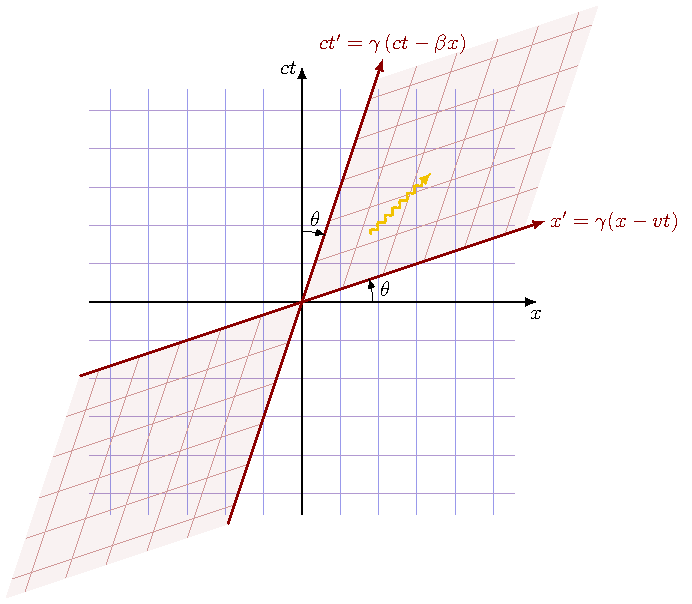
\includegraphics[page=1,width=7.8cm]{minkowski_diagrams.pdf}}
					\label{subfig:lorentz}
					\;
					\subfloat[inverse \textsc{Lorentz} transform\\ according to \autoref{eq:inverselorentz}]{\includegraphics[page=2,width=7.8cm]{minkowski_diagrams.pdf}}
					\label{subfig:inverselorentz}
					\caption{\textsc{Minkowski} diagram as most common visualization of a \textsc{Lorentz} boost along the $x$-axis. This figure visualizes the in \autoref{subsec:minkowski} explicated conncetions. Adapted from \textcite{neutelings}.}
					\label{fig:lorentz}
				\end{figure}
			
			\subsection{Time dilation}
				Consider a clock at rest in $\mathcal S'$, i.e.\ at fixed $x'$. Two ticks are events with coordinates $(x',t_1')$ and $(x',t_2')$ so $\Delta x'=0$ and the proper time between ticks is $\Delta \tau = \Delta t'$. Transforming to $\mathcal S$ using \autoref{eq:inverselorentz} we obtain for the time interval measured in $\mathcal S$
				\begin{equation}
					\boxed{\Delta t = \gamma\,\Delta t'} = \gamma\,\Delta \tau.
					\label{eq:timedilation}
				\end{equation}
				Thus a moving clock (velocity $v$ relative to $\mathcal S$) is measured to run slower by the factor $\gamma$ (time dilation). In words: the time between two events at the same place in the clock's rest frame is longer when observed from a frame in which the clock moves.
			
			\subsection{Length contraction}
			\label{subsec:lengthcontraction}
			
				Let a rod be at rest in $\mathcal S'$ with proper length $L_0 = x_2' - x_1'$, where $x_1',x_2'$ are the (time-independent) endpoint coordinates in $\mathcal S'$. To measure the length in $\mathcal S$ one records the positions of both ends \emph{simultaneously} in $\mathcal S$ at some time $t$; the measured length is $L = x_2 - x_1$ with the same $t$ for both endpoints. Using the inverse Lorentz spatial transform according to \autoref{eq:lorentz} for two events with the same $t$ we get
				$$x_2' - x_1' = \gamma\,(x_2 - x_1) \quad\Rightarrow\quad L_0 = \gamma\,L.$$
				Hence the length measured in $\mathcal S$ is
				\begin{equation}
					\boxed{L = \frac{L_0}{\gamma}}.
					\label{eq:lengthcontraction}
				\end{equation}
				The rod moving with speed $v$ appears contracted along the direction of motion by the factor $1/\gamma$.
			
			\subsection{Geometric intuition in the diagram}
			\label{subsec:minkowskiinterpretation}
			
				In the Minkowski diagram in \autoref{fig:lorentz}: (i) time dilation corresponds to comparing the coordinate time interval along a tilted worldline (moving clock) with the interval along the vertical axis (rest clock) — the projected time on the vertical axis is multiplied by $\gamma$; (ii) length contraction arises because simultaneity lines in different frames are tilted with respect to each other: the slice that is simultaneous in the lab intersects the worldtubes of the rod at a smaller spatial separation than the slice simultaneous in the rod's rest frame.
			
				\paragraph{Note on proper quantities.}
					The proper time $\Delta\tau$ is the time between two timelike-separated events measured in the frame where they occur at the same place. The proper length $L_0$ is the length measured in the frame where the object is at rest. These are invariant definitions; measured (coordinate) times and lengths depend on the observer's frame via the Lorentz transformation.
		
			\subsection{Other definitions}
			\label{subsec:otherdefs}
	
				\begin{relveladd}
					\begin{equation}
						u'=\frac{u-v}{1-\dfrac{uv}{c^2}},\qquad
						u=\frac{u'+v}{1+\dfrac{u'v}{c^2}}.
						\label{eq:relveladd}
					\end{equation}
				\end{relveladd}
				
				derived in \textcite[p.~90-91]{Demtroeder1}.
			
				\begin{minkinterval}
					\begin{equation}
						s^2 = c^2 t^2 - x^2 - y^2 - z^2.
						\label{eq:minkowski}
					\end{equation}
				\end{minkinterval}
				The Lorentz transformation preserves $s^2$ \cite{Griffiths}. In $(ct,x,y,z)$ the boost in $x$-direction reads
				\begin{equation}
					\Lambda(\beta)=
					\begin{pmatrix}
						\gamma & -\gamma\beta & 0 & 0\\
						-\gamma\beta & \gamma & 0 & 0\\
						0&0&1&0\\
						0&0&0&1
					\end{pmatrix},
					\quad
					\text{with }\;
					\begin{pmatrix} ct' \\ x' \\ y' \\ z' \end{pmatrix}
					=\Lambda(\beta)\begin{pmatrix} ct \\ x \\ y \\ z \end{pmatrix}.
				\end{equation}
				
	\FloatBarrier
	\clearpage
	
	\printbibliography
	
	\newpage
	
	\pagenumbering{Roman}
	\appendix
	\setcounter{tocdepth}{1}
	\setcounter{table}{0}
	\setcounter{equation}{0}
	\setcounter{figure}{0}
\end{document}